\chapter{Wykorzystane narzędzia}
\label{cha:narzedzia}

Celem obecnego rozdziału jest opisanie wykorzystanych do implementacji systemu narzędzi, takich jak platforma sprzętowa, biblioteki programowe, środowisko programistyczne.

\section{Platforma sprzętowa nRF52833}

Do projektu wykorzystano układ Nordic Semiconductor nRF52833 z serii nRF52.

\subsection{Charakterystyka układu}

    Platforma nRF52833 to SoC (ang. \textit{System on Chip}) wyposażony w 64 MHz CPU (ang. \textit{Central Processing Unit}) z rdzeniem z rodziny ARM Cortex-M4 oraz jednostką FPU (ang. \textit{Floating Point Unit}) \cite{nrf52833-characteristics}.
    Układ posiada 512 kB pamięci nieulotnej flash oraz 128 kB pamięci operacyjnej RAM (ang. \textit{Random Access Memory}).

    SoC zawiera radiowy układ nadawczo-odbiorczy (ang. \textit{Transreceiver}), umożliwiający odbiór ramek IEEE 802.15.4-2006, co jest kluczowe do uruchomienia aplikacji działającej na stosie Thread.

    Według zapewnień producenta platforma nRF52833 może zostać wykorzystana do zastosowań Smart-Home lub przemysłowego IoT i pracować jako czujnik, lub kontroler \cite{nrf52833-characteristics}.

    Do procesu rozwijania oprogramowania, wykorzystano płytkę ewaluacyjną nRF52833 DK, której schemat blokowy przedstawiono na Rysunku \ref{fig:nrf8233-block-diagram}.

    \begin{figure}[H]
        \centering
        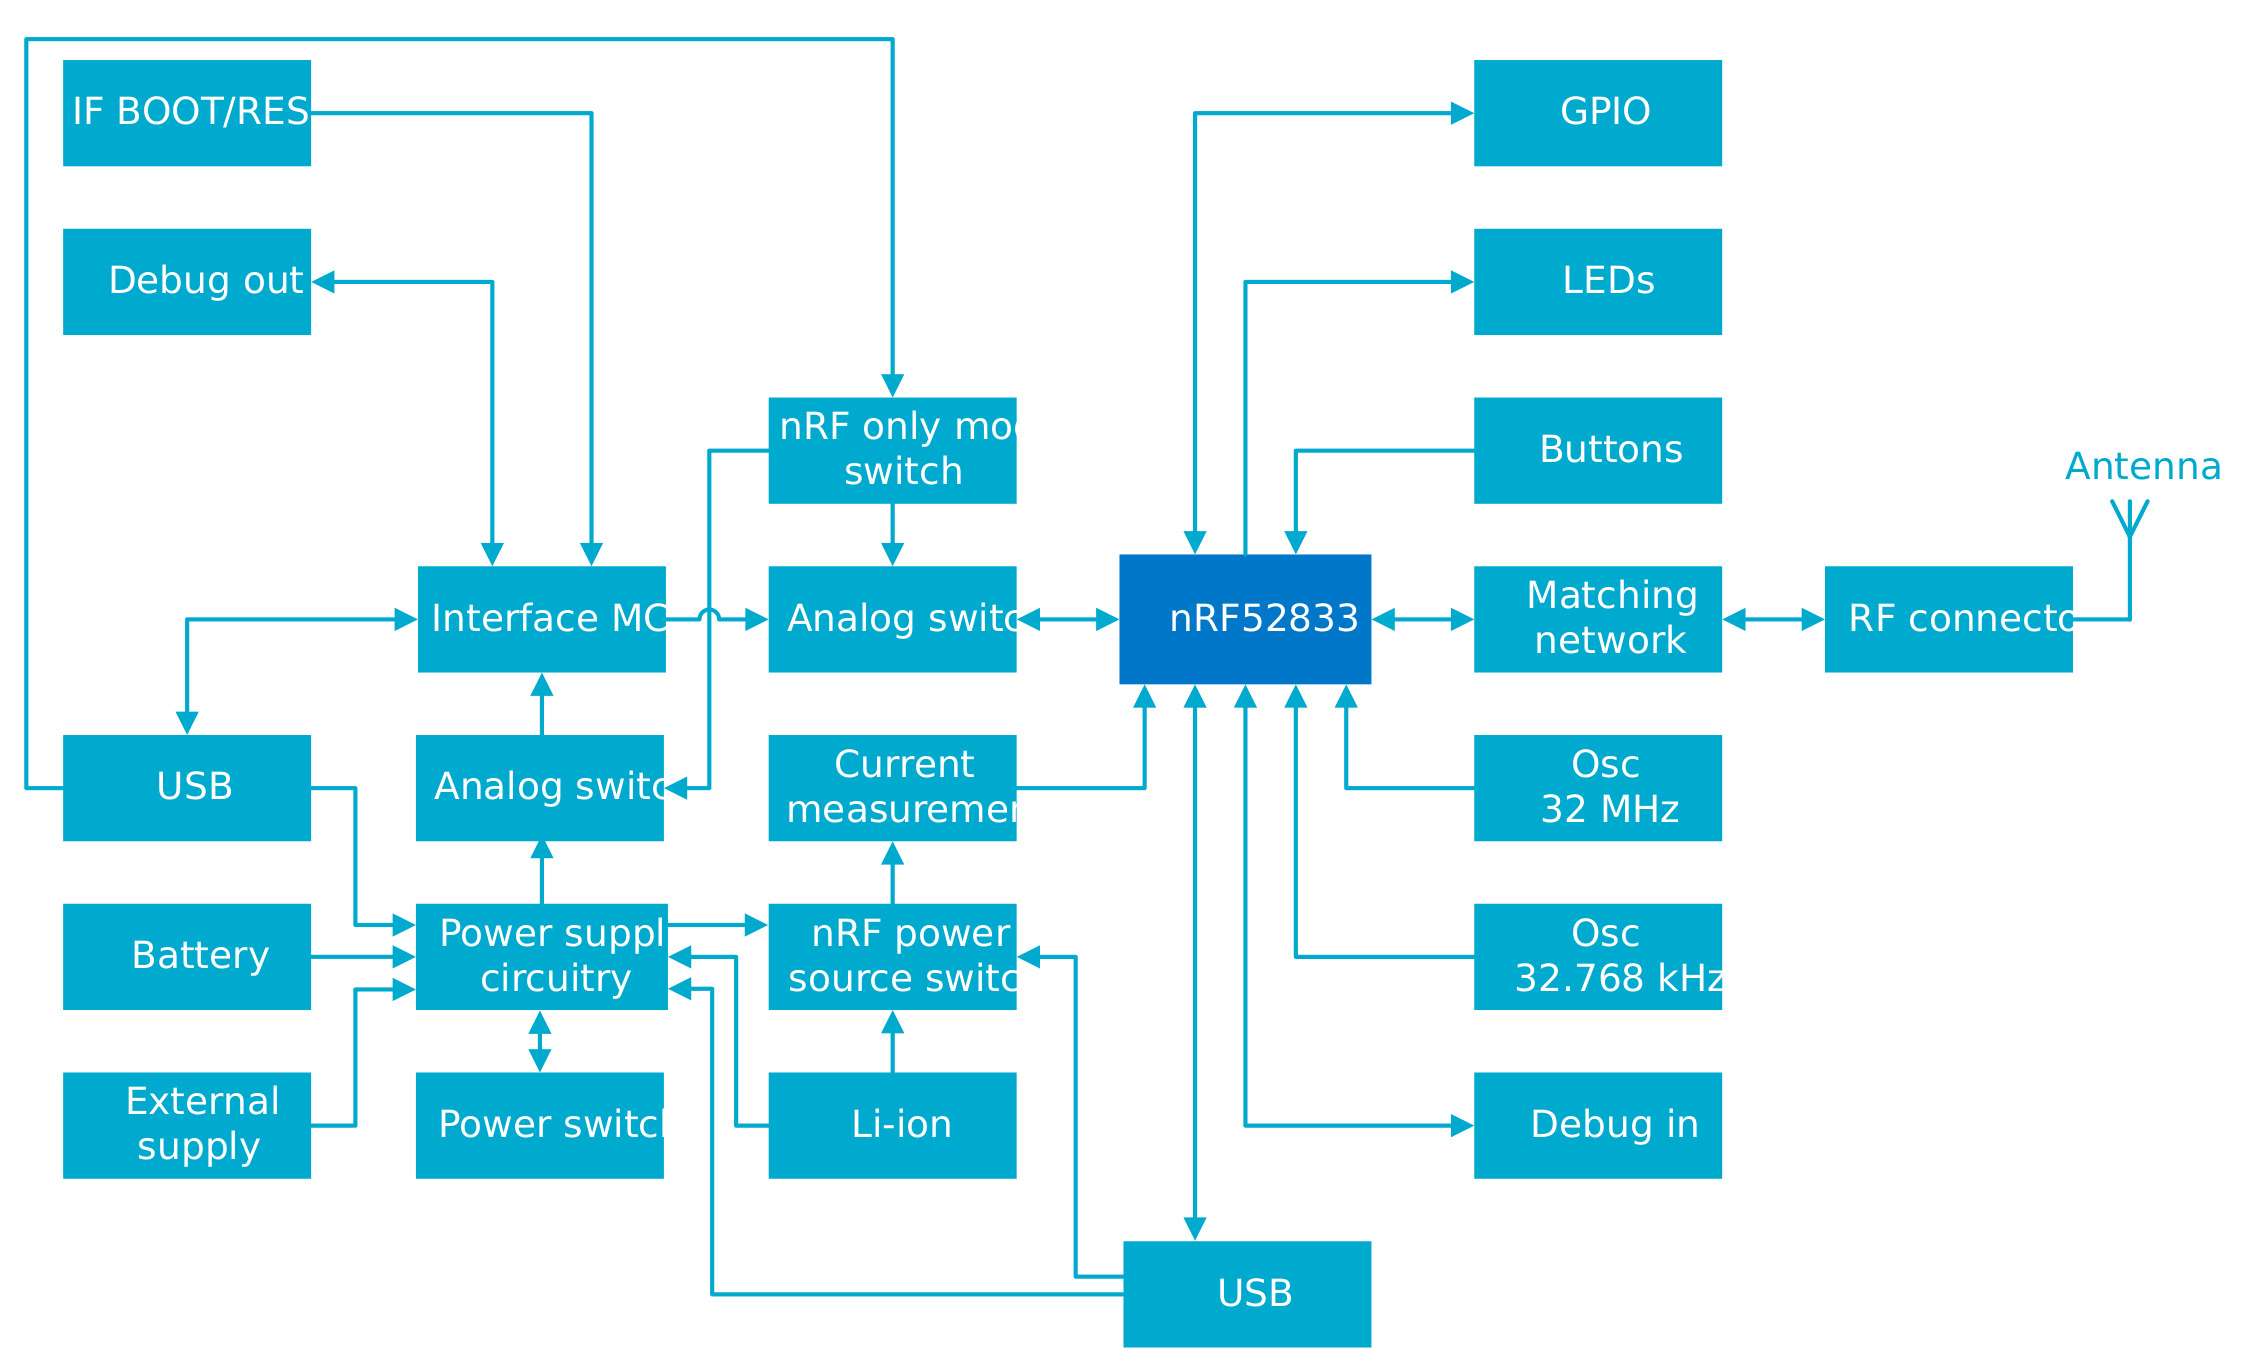
\includegraphics[width=0.8\linewidth]{graphics/external/nrf52833DK_block_diagram.jpg}
        \caption{Schemat blokowy płytki ewaluacyjnej nRF52833 DK \cite{nrf52833-diagram}.}
        \label{fig:nrf8233-block-diagram}
    \end{figure}

\subsection{Narzędzia producenta}
\label{subsec:producer-tools}

    Do tworzenia oprogramowania wykorzystano zestaw narzędzi nRF Connect SDK \cite{nrf-connect}. Stworzone przez Nordic Semiconductor SDK (ang. \textit{Software Development Kit}) jest dedykowane do tworzenia aplikacji, wykorzystujących transmisję bezprzewodową małej mocy. nRF Connect SDK opiera się między innymi, na urządzeniach z serii nRF52 oraz wspiera rozwój oprogramowania w środowisku Microsoft Windows.

    nRF Connect SDK udostępnia system operacyjny czasu rzeczywistego Zephyr oraz przykładowe kody źródłowe aplikacji na nim opartych. Ponadto zestaw narzędzi integruje szereg bibliotek i sterowników z zakresu komunikacji bezprzewodowej, które umożliwiają przyjazne użytkownikowi wdrożenie we własnych aplikacjach, a w szczególności dotyczące technologii:
    \begin{itemize}
        \item Thread,
        \item CoAP (ang. \textit{Constrained Application Protocol}),
        \item IPv6,
        \item UDP,
        \item IEEE 802.15.4.
    \end{itemize}

    W projekcie systemu wykorzystano nRF Connect SDK w wersji 2.4.0.

    Podczas tworzenia oprogramowania, użyto również zapewnione przez Nordic Semiconductor rozszerzenie do edytora tekstu Visual Studio Code \cite{nrf-ide}, który umożliwia tworzenie, konfigurowanie i budowanie aplikacji dedykowanych dla platform Nordic Semiconductor oraz debugowanie i programowanie urządzeń z serii nRF52. 

\section{Openthread}

    OpenThread to upubliczniona, oparta na licencji BSD-3 implementacja stosu Thread, stworzona przez Google. Projekt OpenThread jest wspierany przez, między innymi, Nordic Semiconductor. Stos OpenThread wraz z platformą sprzętową nRF52833 posiada certyfikat \textit{Thread Certified Component} \cite{nrf52833-tcc}, co świadczy o pełnej zgodności ze standardem Thread oraz spełnieniu dodatkowych wymogów wyszczególnionych w specyfikacji \cite{thread-1.3.0}. Implementacja OpenThread wraz z API (ang. \textit{Application Programming Interface}) jest uwzględniona w nRF Connect SDK przedstawionym w podsekcji \ref{subsec:producer-tools}.

    Poza implementacją stosu Thread OpenThread dostarcza dodatkowe narzędzia pomocne przy rozwoju systemów opartych o implementację Thread. Jednym z nich jest aplikacja Rutera Brzegowego OTBR (ang. \textit{OpenThread Border Router}) \cite{openthread-br}.